\documentclass[pdf]{beamer}
\mode<presentation>{}

\usetheme{metropolis}
\usepackage{graphicx}

\title{Evaluating the Capabilities of Lattice Boltzmann Method for non-Newtonian and Free-surface Flows towards Applications in Wellbore Cementing}
\author{Matthew Grasinger}
\date{July 21st, 2016}
\institute{University of Pittsburgh}

\begin{document}

\begin{frame}
\titlepage
\end{frame}

\newcommand{\pw}{0.4\textwidth}
\newcommand{\ph}{0.4\textheight}

\section{Introduction}

\begin{frame}{Non-Newtonian Fluids}
  \begin{table}
    \centering
  \begin{tabular}{cc}
    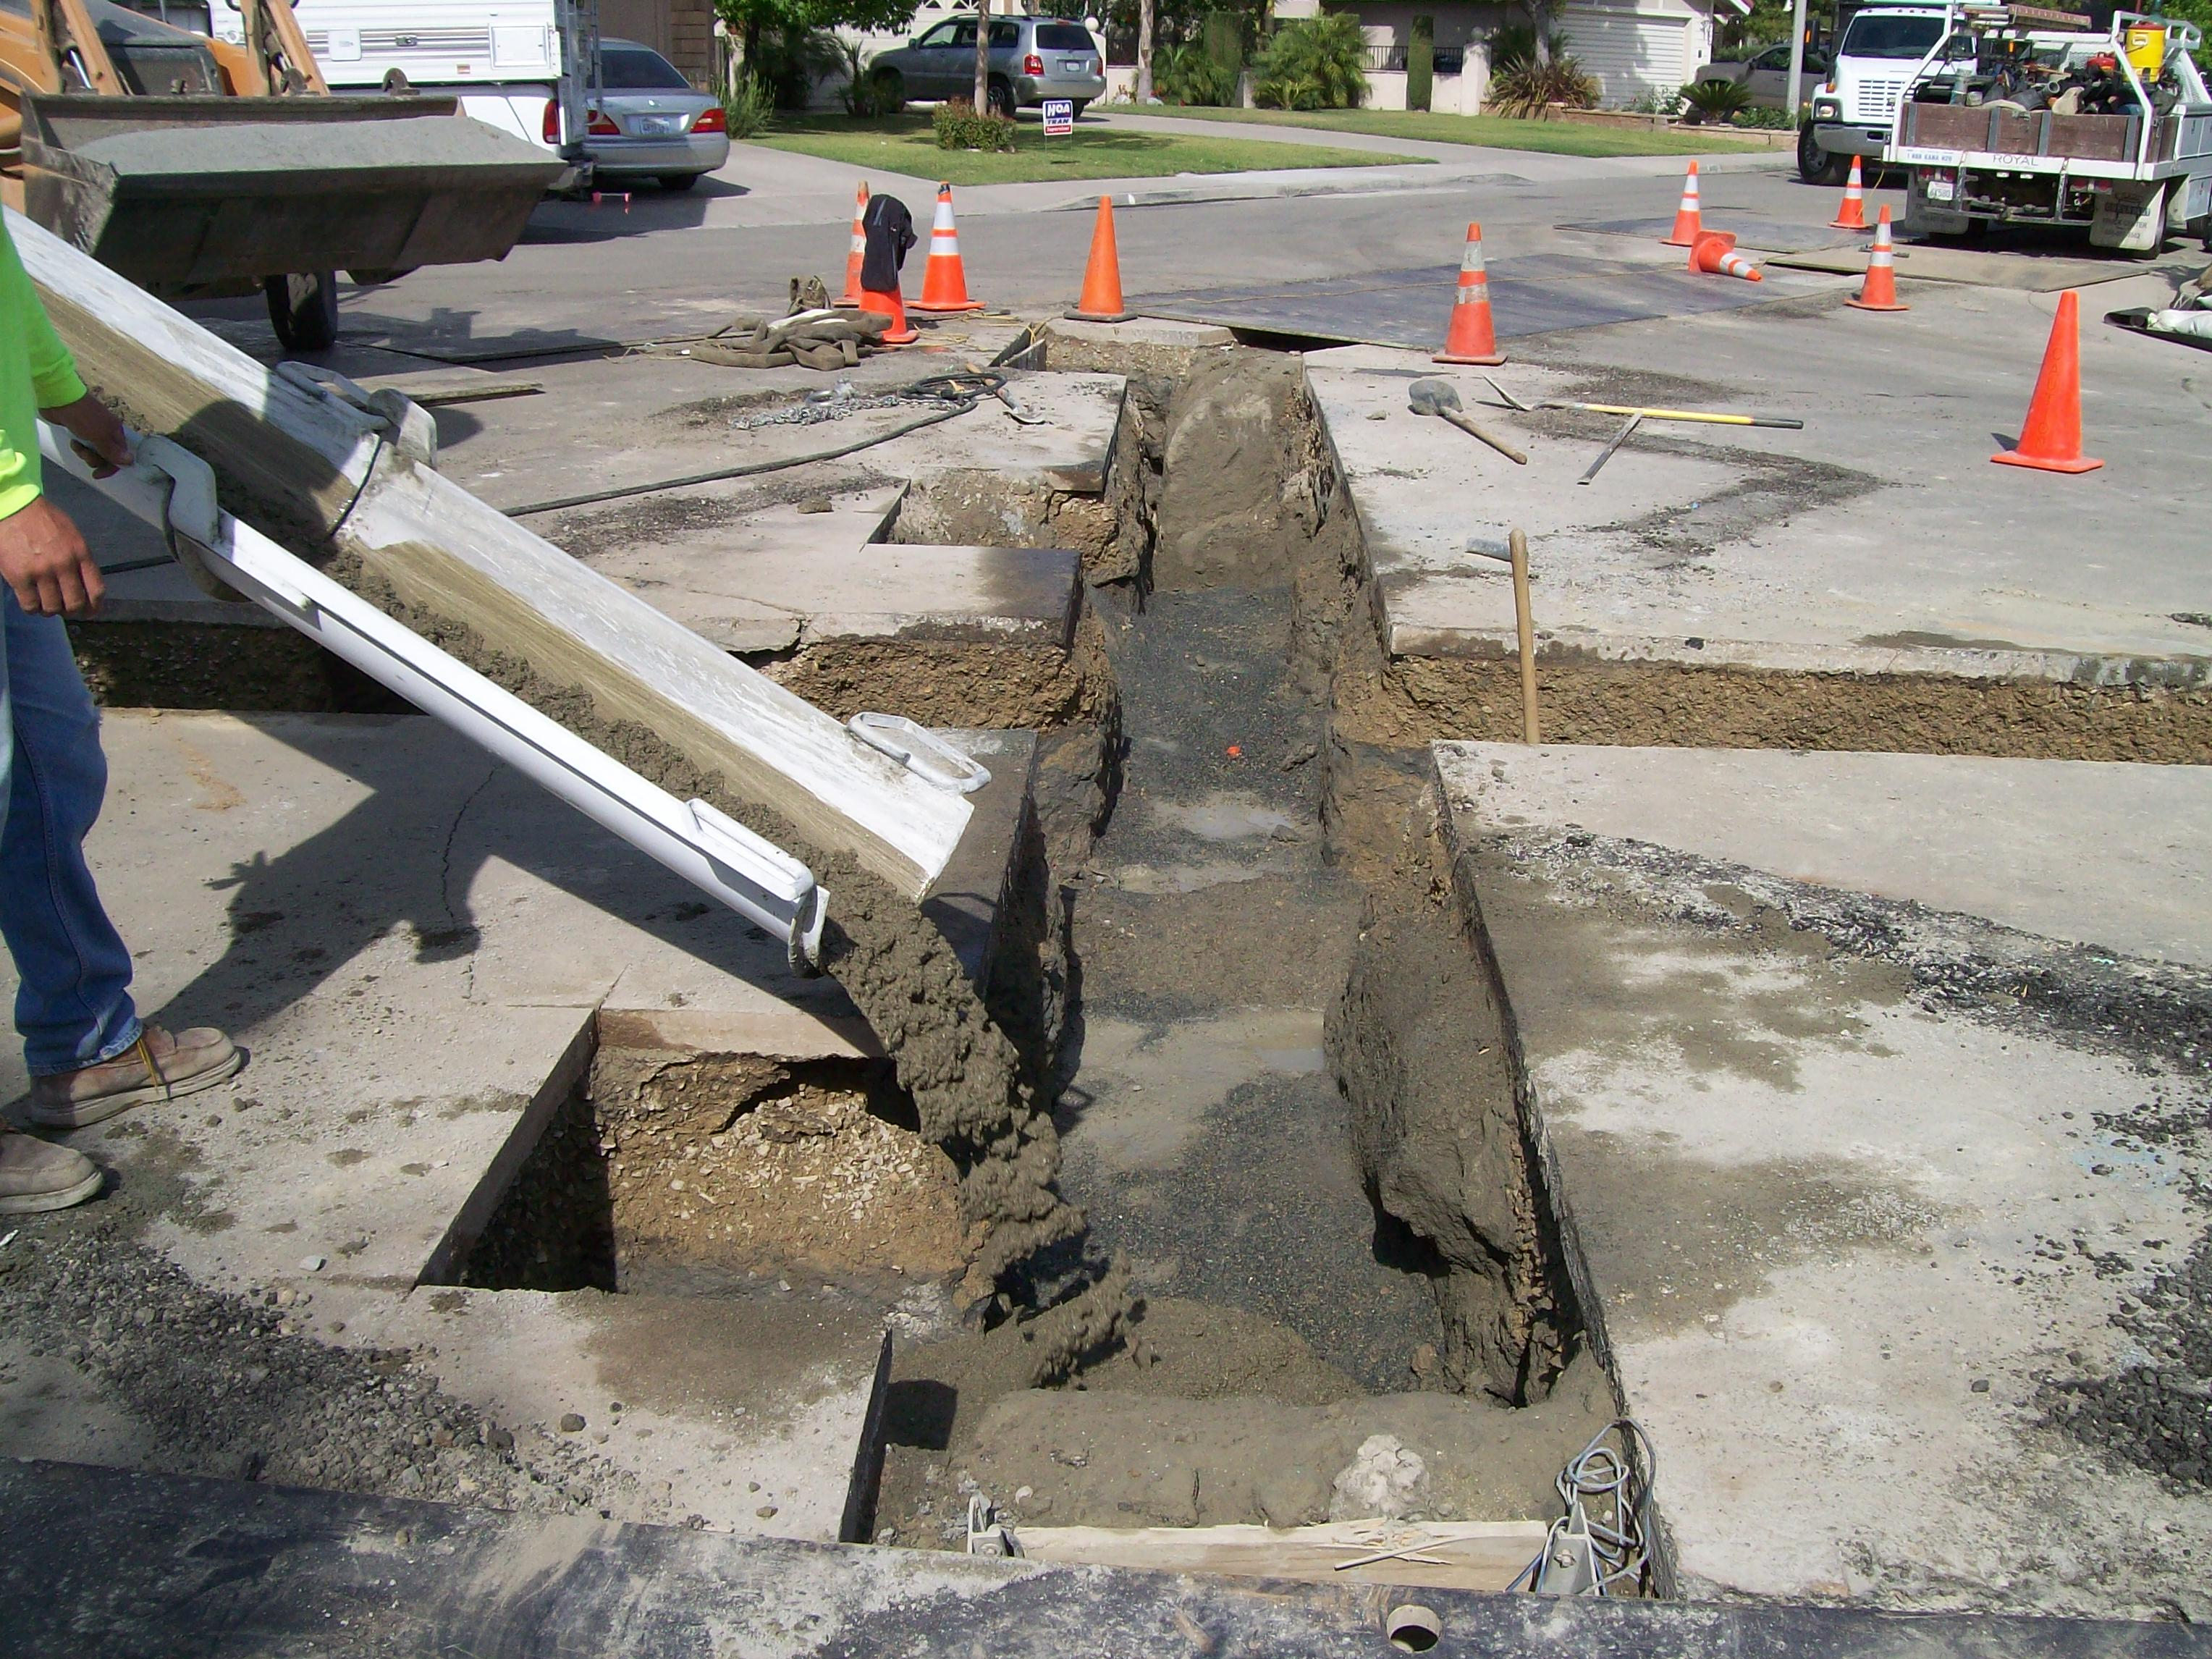
\includegraphics[width=\pw, height=\ph, keepaspectratio]{figs/slurry-backfill} & 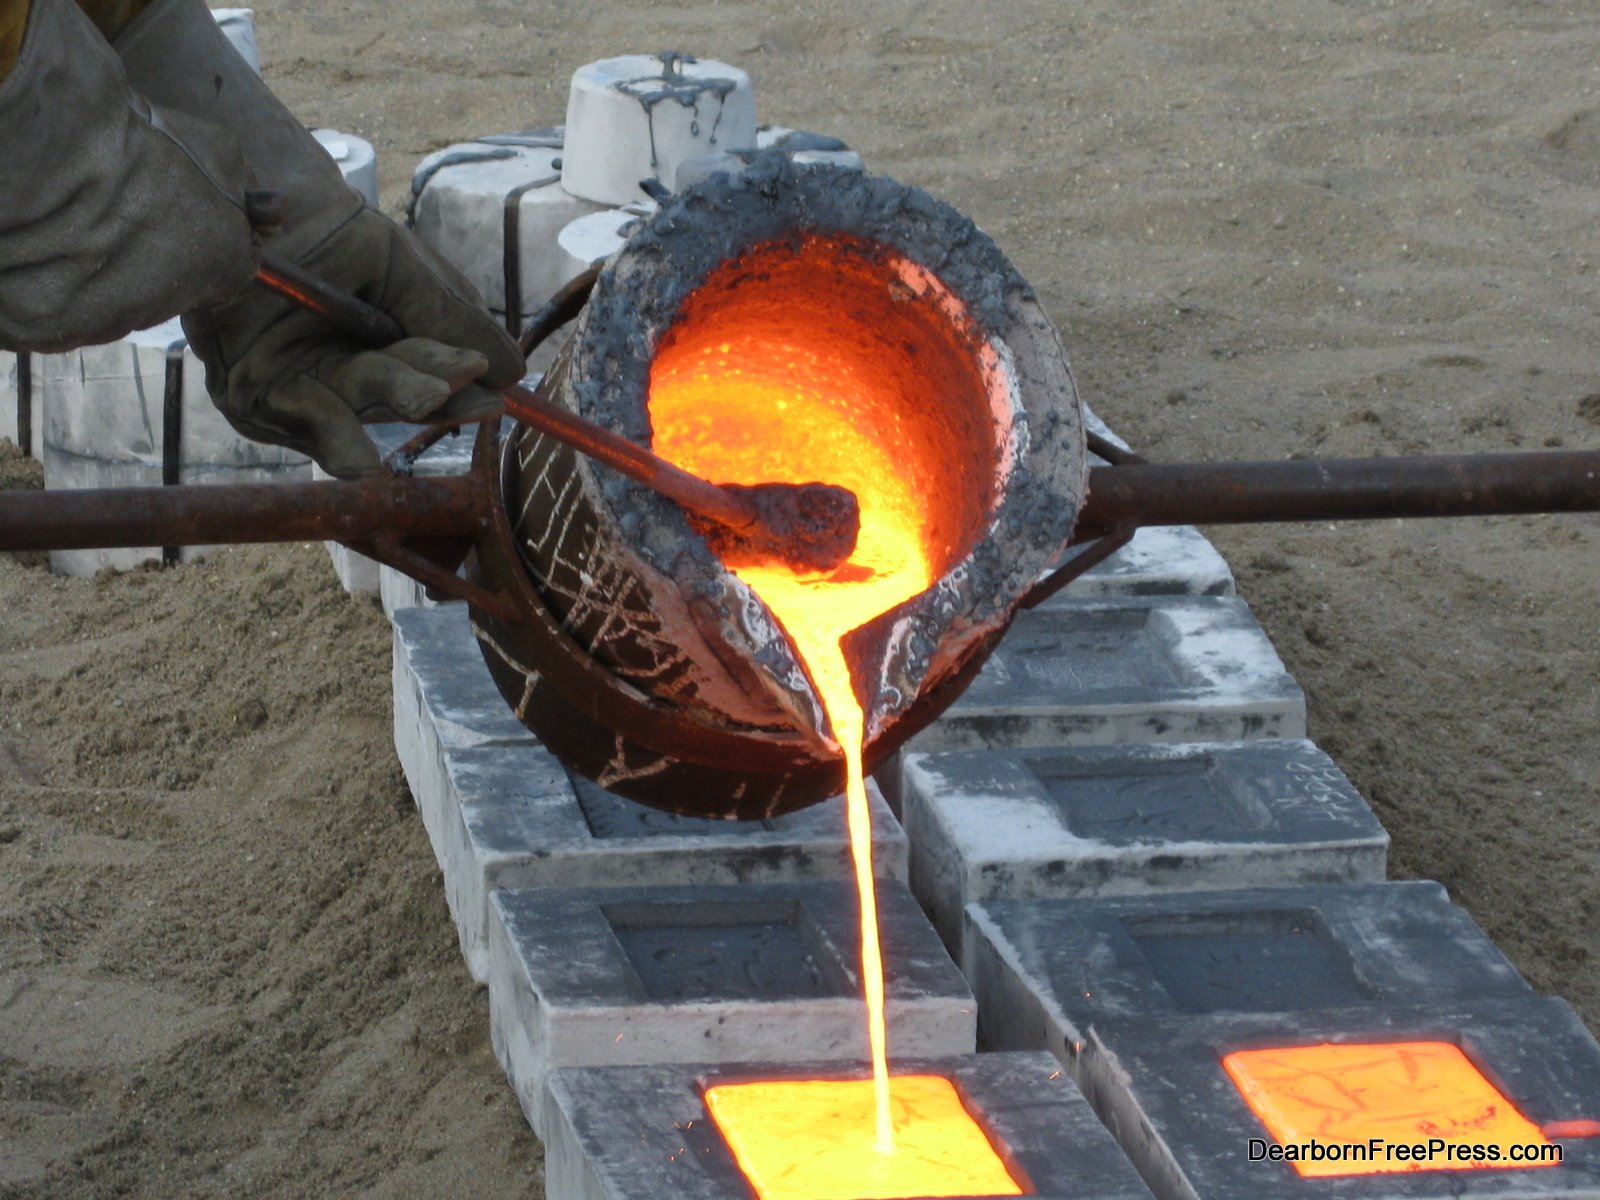
\includegraphics[width=\pw, height=\ph, keepaspectratio]{figs/molten-metal} \\
    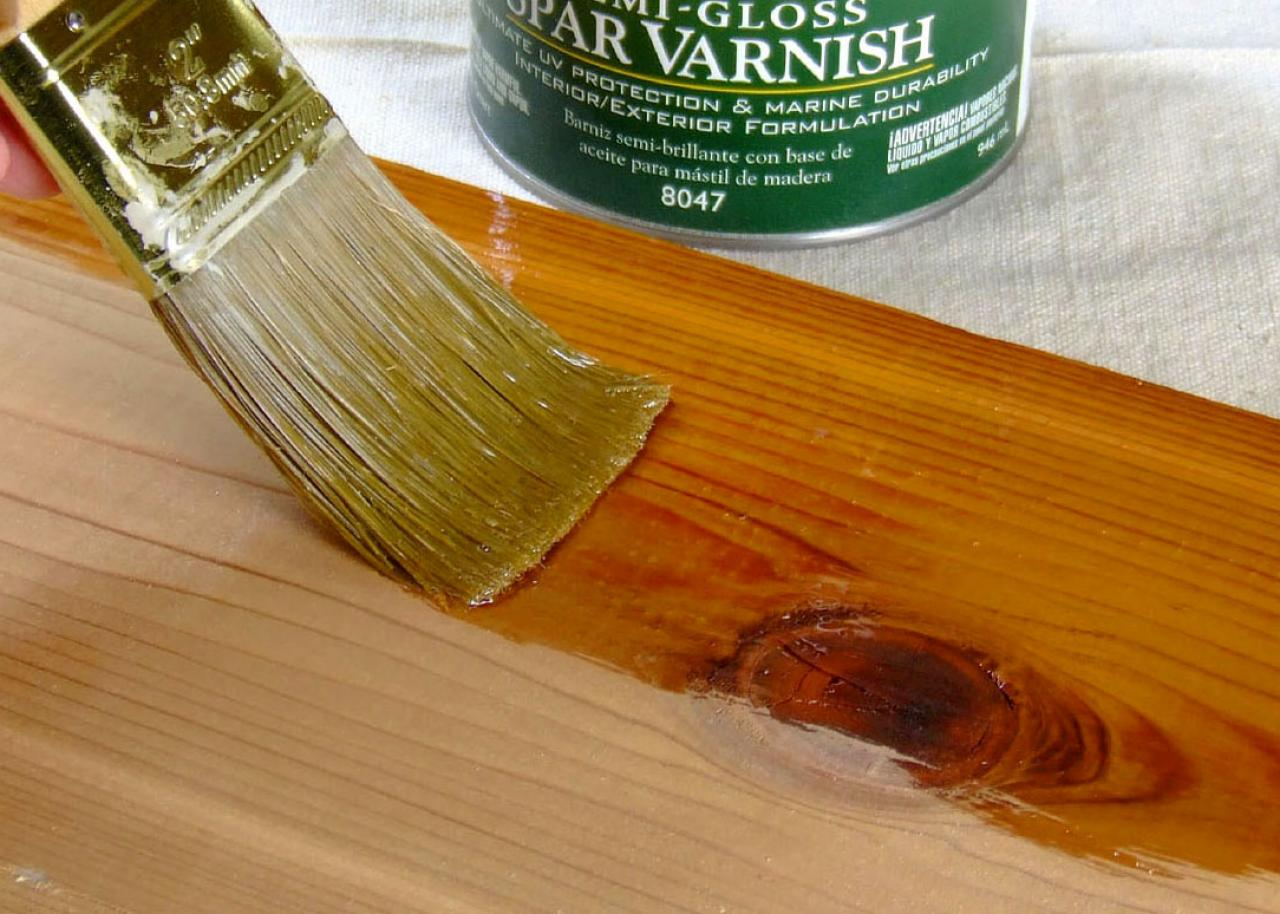
\includegraphics[width=\pw, height=\ph, keepaspectratio]{figs/varnish} & 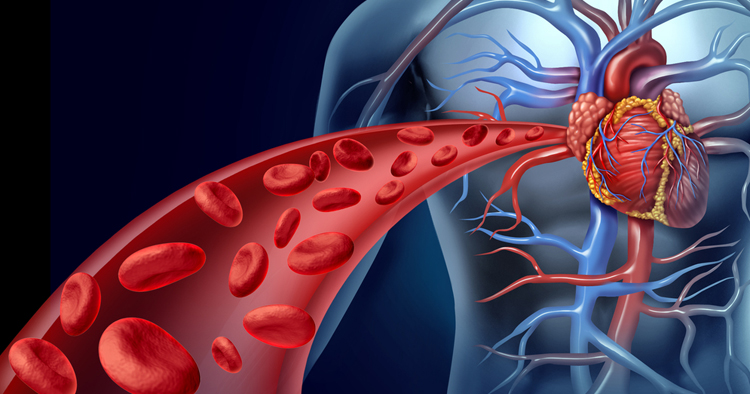
\includegraphics[width=\pw, height=\ph, keepaspectratio]{figs/blood-circulation}
\end{tabular}
\end{table}
\end{frame}

\end{document}
